\section{Results and Discussion} \label{sec:results}

We now present the results of the experiements mentioned in the previous section, as well as their significance.

\subsection{Billion-Tip Reconstruction}

\begin{figure}

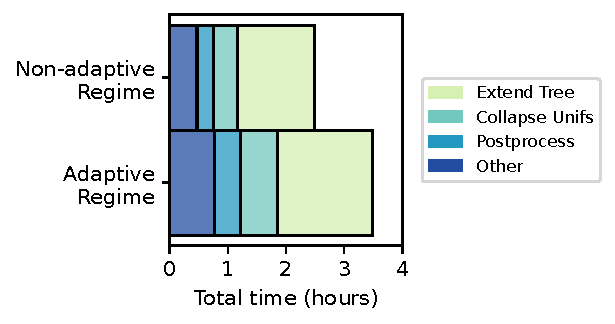
\includegraphics[width=3in]{binder/binder-2025_03_13_preliminary_billion_tip_reconstruction_graphing.ipynb/binder/teeplots/viz=plot-billion-tip-reconstruction-stack+ext=.pdf}

\caption{\textbf{Billion-tip reconstruction times.} TODO.}
\label{fig:billion-tip-time}
\end{figure}


\subsection{Runtime Comparison}

A direct comparison between the naive trie-based and the optimized shortcut table-based approches highlights the massive savings achieved by the new algorithm. As seen in Figure~\ref{fig:comparison}, the original algorithm explodes in runtime, whereas the new algorithm performs so well that there is no clear increase in runtime.

\begin{center}
\begin{figure}[h]
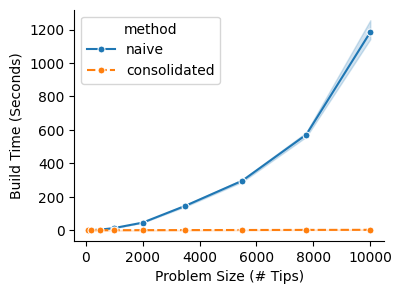
\includegraphics[width=\linewidth]{img/time_by_tips.png}
\caption{
\textbf{Microbenchmark comparison of naive trie and shortcut table algorithms.}
\small
Naive approach appears to exhibit superlinear scaling.
Shaded bands are 95\% confidence intervals, NUM\_TODO samples per observation.
}
\label{fig:comparison}
\end{figure}
\end{center}

The naive and optimized algorithms were implemented with all things constant except for two details: the optimized algorithm used a search table and included shortcut optimizations. Because a search table is merely a different data structure used for a tree (an alternative to using a node-pointer approach), with equivalent time complexities for all operations, one could expect this change to result in a constant speedup (if any) between the two algorithms.

Because this result is not by a constant factor, we can assume that a majority of the speedup came from the shortcuts saving a significant amount of work that was unncessarily done in the naive approach. 

\subsection{Asymptotic Results} \label{sec:results:asymptotic}

